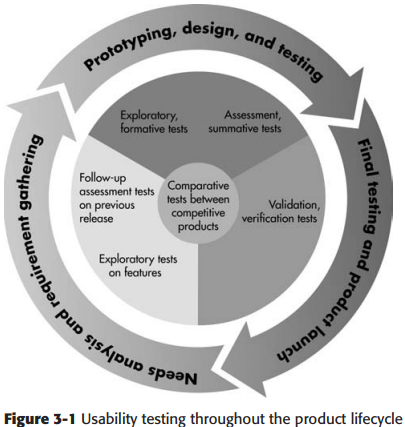
\includegraphics[width=\linewidth]{figures/evaltechcycle.png}

\subsection{Exploratory study}
\begin{itemize}
	\item When / Objective
	\begin{itemize}
		\item Early in development.
		\item Used to examine effectiveness of high-level design aspects, such as: Does the design support user tasks? Does the design communicate the intended workflow properly? 
		\item Used as the foundation of future design work, and is thus important.
	\end{itemize}
	\item Methodology
	\begin{itemize}
		\item Typically conducted using prototypes implementing just what's needed for the test scenario.
		\item Think-aloud testing useful, to gather qualitative data on user thought processes and behavior.
	\end{itemize}
\end{itemize}
\subsection{Assesment / Summative test}
\begin{itemize}
	\item When / Objective
	\begin{itemize}
		\item Early or midways in development, after fundamental design decisions have been made.
		\item Seeks to assess whether the design decisions have been implemented well. Assumes that design decisions are well founded. Looks for specific usability problems while conducting specific tasks
	\end{itemize}
	\item Methodology (compared to exploratory)
	\begin{itemize}
		\item Users perform tasks rather than walking through screens.
		\item Interaction with test moderator is lessened.
		\item Quantitative data will be collected, as the test is about collecting concrete information.
	\end{itemize}
\end{itemize}
\subsection{Validation / Verification test}
\begin{itemize}
	\item When / Objective
	\begin{itemize}
		\item Late in the development cycle.
		\item Compares the product to some specified benchmark or standard. In verification test, verify that previously discovered usability problems have been resolved and that new ones haven't been introduced since. 
		\item Often stated in terms of performance criteria such as efficiency.
		\item Also used to evaluate how the different components in a system work together, that is, validation tests are often integrated tests.
	\end{itemize}
	\item Methodology
	\begin{itemize}
		\item A benchmark is determined beforehand, either in terms of specific error counts or time measures, or simply eliminating earlier problems.
		\item Minimal interaction with test moderator.
		\item High emphasis on quantitative data and how this data is used. 
	\end{itemize}
\end{itemize}
\subsection{Comparison test (AB testing)}
\begin{itemize}
	\item When / Objective
	\begin{itemize}
		\item Any time during development.
		\item Early on: Compare different styles of interface design.
		\item Midways: Compare different implementations of a specific element (does text or an image/icon work better?)
		\item Late: Compare product to competitors
	\end{itemize}
	\item Methodology
	\begin{itemize}
		\item Typically a variant of the other test types, but where users are presented with different versions side-by-side.
		\item The amount of varying dimensions should be considered. If statistically valid results are desired, the designs must vary in one way only.
		\item Typically, the ''best'' design is a combination of the different designs, rather than there being a clear winner. 
		\item In exploratory tests, the alternatives should be radically different if possible, to get as many different ideas as possible. 
		\item Test persons are asked to compare designs and try to explain what makes one design better than another. 
	\end{itemize}
\end{itemize}


